% generated by make_figs.py from a real FastBandSolver run; do not edit by hand
\begin{figure}[p]
\centering
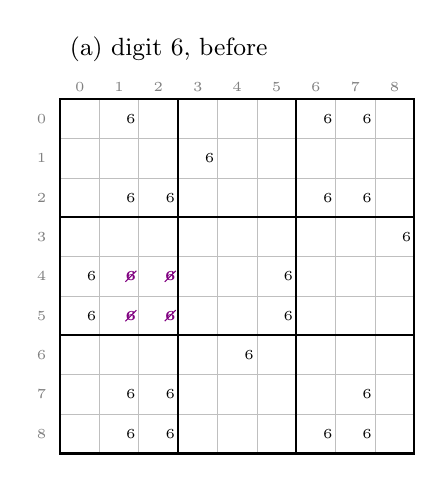
\begin{tikzpicture}[x=1cm,y=1cm]
\node[anchor=south west,font=\small] at (0,4.850) {(a) digit 6, before};
\node[font=\tiny,text=black,inner sep=0] at (0.900,4.250) {6};
\node[font=\tiny,text=black,inner sep=0] at (3.400,4.250) {6};
\node[font=\tiny,text=black,inner sep=0] at (3.900,4.250) {6};
\node[font=\tiny,text=black,inner sep=0] at (1.900,3.750) {6};
\node[font=\tiny,text=black,inner sep=0] at (0.900,3.250) {6};
\node[font=\tiny,text=black,inner sep=0] at (1.400,3.250) {6};
\node[font=\tiny,text=black,inner sep=0] at (3.400,3.250) {6};
\node[font=\tiny,text=black,inner sep=0] at (3.900,3.250) {6};
\node[font=\tiny,text=black,inner sep=0] at (4.400,2.750) {6};
\node[font=\tiny,text=black,inner sep=0] at (0.400,2.250) {6};
\node[font=\tiny\bfseries,text=violet,inner sep=0] at (0.900,2.250) {6};
\draw[violet,thin] (0.830,2.180) -- (0.970,2.320);
\node[font=\tiny\bfseries,text=violet,inner sep=0] at (1.400,2.250) {6};
\draw[violet,thin] (1.330,2.180) -- (1.470,2.320);
\node[font=\tiny,text=black,inner sep=0] at (2.900,2.250) {6};
\node[font=\tiny,text=black,inner sep=0] at (0.400,1.750) {6};
\node[font=\tiny\bfseries,text=violet,inner sep=0] at (0.900,1.750) {6};
\draw[violet,thin] (0.830,1.680) -- (0.970,1.820);
\node[font=\tiny\bfseries,text=violet,inner sep=0] at (1.400,1.750) {6};
\draw[violet,thin] (1.330,1.680) -- (1.470,1.820);
\node[font=\tiny,text=black,inner sep=0] at (2.900,1.750) {6};
\node[font=\tiny,text=black,inner sep=0] at (2.400,1.250) {6};
\node[font=\tiny,text=black,inner sep=0] at (0.900,0.750) {6};
\node[font=\tiny,text=black,inner sep=0] at (1.400,0.750) {6};
\node[font=\tiny,text=black,inner sep=0] at (3.900,0.750) {6};
\node[font=\tiny,text=black,inner sep=0] at (0.900,0.250) {6};
\node[font=\tiny,text=black,inner sep=0] at (1.400,0.250) {6};
\node[font=\tiny,text=black,inner sep=0] at (3.400,0.250) {6};
\node[font=\tiny,text=black,inner sep=0] at (3.900,0.250) {6};
\draw[step=0.5,gray!50,very thin] (0,0) grid (4.500,4.500);
\draw[thick] (1.500,0) -- (1.500,4.500);
\draw[thick] (3.000,0) -- (3.000,4.500);
\draw[thick] (0,3.000) -- (4.500,3.000);
\draw[thick] (0,1.500) -- (4.500,1.500);
\draw[thick] (0,0) rectangle (4.500,4.500);
\node[font=\tiny,text=gray] at (0.250,4.650) {0};
\node[font=\tiny,text=gray] at (0.750,4.650) {1};
\node[font=\tiny,text=gray] at (1.250,4.650) {2};
\node[font=\tiny,text=gray] at (1.750,4.650) {3};
\node[font=\tiny,text=gray] at (2.250,4.650) {4};
\node[font=\tiny,text=gray] at (2.750,4.650) {5};
\node[font=\tiny,text=gray] at (3.250,4.650) {6};
\node[font=\tiny,text=gray] at (3.750,4.650) {7};
\node[font=\tiny,text=gray] at (4.250,4.650) {8};
\node[font=\tiny,text=gray,anchor=east] at (-0.05,4.250) {0};
\node[font=\tiny,text=gray,anchor=east] at (-0.05,3.750) {1};
\node[font=\tiny,text=gray,anchor=east] at (-0.05,3.250) {2};
\node[font=\tiny,text=gray,anchor=east] at (-0.05,2.750) {3};
\node[font=\tiny,text=gray,anchor=east] at (-0.05,2.250) {4};
\node[font=\tiny,text=gray,anchor=east] at (-0.05,1.750) {5};
\node[font=\tiny,text=gray,anchor=east] at (-0.05,1.250) {6};
\node[font=\tiny,text=gray,anchor=east] at (-0.05,0.750) {7};
\node[font=\tiny,text=gray,anchor=east] at (-0.05,0.250) {8};
\end{tikzpicture}
\hspace{1cm}
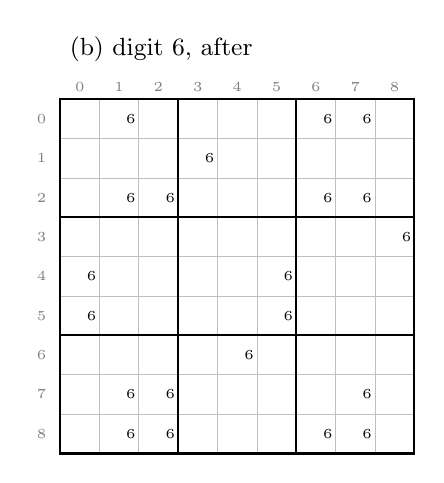
\begin{tikzpicture}[x=1cm,y=1cm]
\node[anchor=south west,font=\small] at (0,4.850) {(b) digit 6, after};
\node[font=\tiny,text=black,inner sep=0] at (0.900,4.250) {6};
\node[font=\tiny,text=black,inner sep=0] at (3.400,4.250) {6};
\node[font=\tiny,text=black,inner sep=0] at (3.900,4.250) {6};
\node[font=\tiny,text=black,inner sep=0] at (1.900,3.750) {6};
\node[font=\tiny,text=black,inner sep=0] at (0.900,3.250) {6};
\node[font=\tiny,text=black,inner sep=0] at (1.400,3.250) {6};
\node[font=\tiny,text=black,inner sep=0] at (3.400,3.250) {6};
\node[font=\tiny,text=black,inner sep=0] at (3.900,3.250) {6};
\node[font=\tiny,text=black,inner sep=0] at (4.400,2.750) {6};
\node[font=\tiny,text=black,inner sep=0] at (0.400,2.250) {6};
\node[font=\tiny,text=black,inner sep=0] at (2.900,2.250) {6};
\node[font=\tiny,text=black,inner sep=0] at (0.400,1.750) {6};
\node[font=\tiny,text=black,inner sep=0] at (2.900,1.750) {6};
\node[font=\tiny,text=black,inner sep=0] at (2.400,1.250) {6};
\node[font=\tiny,text=black,inner sep=0] at (0.900,0.750) {6};
\node[font=\tiny,text=black,inner sep=0] at (1.400,0.750) {6};
\node[font=\tiny,text=black,inner sep=0] at (3.900,0.750) {6};
\node[font=\tiny,text=black,inner sep=0] at (0.900,0.250) {6};
\node[font=\tiny,text=black,inner sep=0] at (1.400,0.250) {6};
\node[font=\tiny,text=black,inner sep=0] at (3.400,0.250) {6};
\node[font=\tiny,text=black,inner sep=0] at (3.900,0.250) {6};
\draw[step=0.5,gray!50,very thin] (0,0) grid (4.500,4.500);
\draw[thick] (1.500,0) -- (1.500,4.500);
\draw[thick] (3.000,0) -- (3.000,4.500);
\draw[thick] (0,3.000) -- (4.500,3.000);
\draw[thick] (0,1.500) -- (4.500,1.500);
\draw[thick] (0,0) rectangle (4.500,4.500);
\node[font=\tiny,text=gray] at (0.250,4.650) {0};
\node[font=\tiny,text=gray] at (0.750,4.650) {1};
\node[font=\tiny,text=gray] at (1.250,4.650) {2};
\node[font=\tiny,text=gray] at (1.750,4.650) {3};
\node[font=\tiny,text=gray] at (2.250,4.650) {4};
\node[font=\tiny,text=gray] at (2.750,4.650) {5};
\node[font=\tiny,text=gray] at (3.250,4.650) {6};
\node[font=\tiny,text=gray] at (3.750,4.650) {7};
\node[font=\tiny,text=gray] at (4.250,4.650) {8};
\node[font=\tiny,text=gray,anchor=east] at (-0.05,4.250) {0};
\node[font=\tiny,text=gray,anchor=east] at (-0.05,3.750) {1};
\node[font=\tiny,text=gray,anchor=east] at (-0.05,3.250) {2};
\node[font=\tiny,text=gray,anchor=east] at (-0.05,2.750) {3};
\node[font=\tiny,text=gray,anchor=east] at (-0.05,2.250) {4};
\node[font=\tiny,text=gray,anchor=east] at (-0.05,1.750) {5};
\node[font=\tiny,text=gray,anchor=east] at (-0.05,1.250) {6};
\node[font=\tiny,text=gray,anchor=east] at (-0.05,0.750) {7};
\node[font=\tiny,text=gray,anchor=east] at (-0.05,0.250) {8};
\end{tikzpicture}
\\[0.5cm]
{\small (c) the tables $B^{6,s}$ (bands $\times$ columns) for stacks 0, 1, 2, before}\\[3pt]
$\begin{array}{c|ccc} & 0 & 1 & 2 \\ \hline \text{band }0 & 0 & \mathbf{1} & \mathbf{1} \\ \text{band }1 & \mathbf{1} & \textcolor{violet}{\mathbf{1}} & \textcolor{violet}{\mathbf{1}} \\ \text{band }2 & 0 & \mathbf{1} & \mathbf{1}\end{array}$\quad$\begin{array}{c|ccc} & 3 & 4 & 5 \\ \hline \text{band }0 & \mathbf{1} & 0 & 0 \\ \text{band }1 & 0 & 0 & \mathbf{1} \\ \text{band }2 & 0 & \mathbf{1} & 0\end{array}$\quad$\begin{array}{c|ccc} & 6 & 7 & 8 \\ \hline \text{band }0 & \mathbf{1} & \mathbf{1} & 0 \\ \text{band }1 & 0 & 0 & \mathbf{1} \\ \text{band }2 & \mathbf{1} & \mathbf{1} & 0\end{array}$
\caption{\textsc{StackRule} (\cref{alg:stack}) for digit 6, the call made inside the band update of \cref{fig:alg-band}. (a), (b): digit 6's candidates over the whole grid; the violet ones are removed. (c): for each stack, a 1 where the band still has digit 6 in that column; entries on some perfect matching are bold, and violet entries are on none. In stack 0, bands 0 and 2 can only use columns 1 and 2, so between them they take both, and band 1 must use the remaining column: it loses columns 1 and 2. That removes 6 from 4 cells. In stacks 1 and 2 every entry is on a perfect matching, so nothing changes there.}
\label{fig:alg-stack}
\end{figure}
